% Generated by Sphinx.
\def\sphinxdocclass{report}
\documentclass[letterpaper,10pt,english]{sphinxmanual}
\usepackage[utf8]{inputenc}
\DeclareUnicodeCharacter{00A0}{\nobreakspace}
\usepackage{cmap}
\usepackage[T1]{fontenc}
\usepackage{babel}
\usepackage{times}
\usepackage[Bjarne]{fncychap}
\usepackage{longtable}
\usepackage{sphinx}
\usepackage{multirow}

\addto\captionsenglish{\renewcommand{\figurename}{Fig. }}
\addto\captionsenglish{\renewcommand{\tablename}{Table }}
\floatname{literal-block}{Listing }



\title{ecoop Documentation}
\date{October 30, 2015}
\release{0.1.1}
\author{Massimo Di Stefano}
\newcommand{\sphinxlogo}{}
\renewcommand{\releasename}{Release}
\makeindex

\makeatletter
\def\PYG@reset{\let\PYG@it=\relax \let\PYG@bf=\relax%
    \let\PYG@ul=\relax \let\PYG@tc=\relax%
    \let\PYG@bc=\relax \let\PYG@ff=\relax}
\def\PYG@tok#1{\csname PYG@tok@#1\endcsname}
\def\PYG@toks#1+{\ifx\relax#1\empty\else%
    \PYG@tok{#1}\expandafter\PYG@toks\fi}
\def\PYG@do#1{\PYG@bc{\PYG@tc{\PYG@ul{%
    \PYG@it{\PYG@bf{\PYG@ff{#1}}}}}}}
\def\PYG#1#2{\PYG@reset\PYG@toks#1+\relax+\PYG@do{#2}}

\expandafter\def\csname PYG@tok@vg\endcsname{\def\PYG@tc##1{\textcolor[rgb]{0.73,0.38,0.84}{##1}}}
\expandafter\def\csname PYG@tok@nd\endcsname{\let\PYG@bf=\textbf\def\PYG@tc##1{\textcolor[rgb]{0.33,0.33,0.33}{##1}}}
\expandafter\def\csname PYG@tok@go\endcsname{\def\PYG@tc##1{\textcolor[rgb]{0.20,0.20,0.20}{##1}}}
\expandafter\def\csname PYG@tok@ss\endcsname{\def\PYG@tc##1{\textcolor[rgb]{0.32,0.47,0.09}{##1}}}
\expandafter\def\csname PYG@tok@nn\endcsname{\let\PYG@bf=\textbf\def\PYG@tc##1{\textcolor[rgb]{0.05,0.52,0.71}{##1}}}
\expandafter\def\csname PYG@tok@kp\endcsname{\def\PYG@tc##1{\textcolor[rgb]{0.00,0.44,0.13}{##1}}}
\expandafter\def\csname PYG@tok@sr\endcsname{\def\PYG@tc##1{\textcolor[rgb]{0.14,0.33,0.53}{##1}}}
\expandafter\def\csname PYG@tok@sc\endcsname{\def\PYG@tc##1{\textcolor[rgb]{0.25,0.44,0.63}{##1}}}
\expandafter\def\csname PYG@tok@gh\endcsname{\let\PYG@bf=\textbf\def\PYG@tc##1{\textcolor[rgb]{0.00,0.00,0.50}{##1}}}
\expandafter\def\csname PYG@tok@s\endcsname{\def\PYG@tc##1{\textcolor[rgb]{0.25,0.44,0.63}{##1}}}
\expandafter\def\csname PYG@tok@cm\endcsname{\let\PYG@it=\textit\def\PYG@tc##1{\textcolor[rgb]{0.25,0.50,0.56}{##1}}}
\expandafter\def\csname PYG@tok@se\endcsname{\let\PYG@bf=\textbf\def\PYG@tc##1{\textcolor[rgb]{0.25,0.44,0.63}{##1}}}
\expandafter\def\csname PYG@tok@gr\endcsname{\def\PYG@tc##1{\textcolor[rgb]{1.00,0.00,0.00}{##1}}}
\expandafter\def\csname PYG@tok@mo\endcsname{\def\PYG@tc##1{\textcolor[rgb]{0.13,0.50,0.31}{##1}}}
\expandafter\def\csname PYG@tok@mf\endcsname{\def\PYG@tc##1{\textcolor[rgb]{0.13,0.50,0.31}{##1}}}
\expandafter\def\csname PYG@tok@ge\endcsname{\let\PYG@it=\textit}
\expandafter\def\csname PYG@tok@il\endcsname{\def\PYG@tc##1{\textcolor[rgb]{0.13,0.50,0.31}{##1}}}
\expandafter\def\csname PYG@tok@nv\endcsname{\def\PYG@tc##1{\textcolor[rgb]{0.73,0.38,0.84}{##1}}}
\expandafter\def\csname PYG@tok@mh\endcsname{\def\PYG@tc##1{\textcolor[rgb]{0.13,0.50,0.31}{##1}}}
\expandafter\def\csname PYG@tok@mb\endcsname{\def\PYG@tc##1{\textcolor[rgb]{0.13,0.50,0.31}{##1}}}
\expandafter\def\csname PYG@tok@c1\endcsname{\let\PYG@it=\textit\def\PYG@tc##1{\textcolor[rgb]{0.25,0.50,0.56}{##1}}}
\expandafter\def\csname PYG@tok@s1\endcsname{\def\PYG@tc##1{\textcolor[rgb]{0.25,0.44,0.63}{##1}}}
\expandafter\def\csname PYG@tok@ne\endcsname{\def\PYG@tc##1{\textcolor[rgb]{0.00,0.44,0.13}{##1}}}
\expandafter\def\csname PYG@tok@sd\endcsname{\let\PYG@it=\textit\def\PYG@tc##1{\textcolor[rgb]{0.25,0.44,0.63}{##1}}}
\expandafter\def\csname PYG@tok@ow\endcsname{\let\PYG@bf=\textbf\def\PYG@tc##1{\textcolor[rgb]{0.00,0.44,0.13}{##1}}}
\expandafter\def\csname PYG@tok@sb\endcsname{\def\PYG@tc##1{\textcolor[rgb]{0.25,0.44,0.63}{##1}}}
\expandafter\def\csname PYG@tok@nb\endcsname{\def\PYG@tc##1{\textcolor[rgb]{0.00,0.44,0.13}{##1}}}
\expandafter\def\csname PYG@tok@gp\endcsname{\let\PYG@bf=\textbf\def\PYG@tc##1{\textcolor[rgb]{0.78,0.36,0.04}{##1}}}
\expandafter\def\csname PYG@tok@gt\endcsname{\def\PYG@tc##1{\textcolor[rgb]{0.00,0.27,0.87}{##1}}}
\expandafter\def\csname PYG@tok@m\endcsname{\def\PYG@tc##1{\textcolor[rgb]{0.13,0.50,0.31}{##1}}}
\expandafter\def\csname PYG@tok@kd\endcsname{\let\PYG@bf=\textbf\def\PYG@tc##1{\textcolor[rgb]{0.00,0.44,0.13}{##1}}}
\expandafter\def\csname PYG@tok@o\endcsname{\def\PYG@tc##1{\textcolor[rgb]{0.40,0.40,0.40}{##1}}}
\expandafter\def\csname PYG@tok@si\endcsname{\let\PYG@it=\textit\def\PYG@tc##1{\textcolor[rgb]{0.44,0.63,0.82}{##1}}}
\expandafter\def\csname PYG@tok@vi\endcsname{\def\PYG@tc##1{\textcolor[rgb]{0.73,0.38,0.84}{##1}}}
\expandafter\def\csname PYG@tok@kt\endcsname{\def\PYG@tc##1{\textcolor[rgb]{0.56,0.13,0.00}{##1}}}
\expandafter\def\csname PYG@tok@kr\endcsname{\let\PYG@bf=\textbf\def\PYG@tc##1{\textcolor[rgb]{0.00,0.44,0.13}{##1}}}
\expandafter\def\csname PYG@tok@w\endcsname{\def\PYG@tc##1{\textcolor[rgb]{0.73,0.73,0.73}{##1}}}
\expandafter\def\csname PYG@tok@sh\endcsname{\def\PYG@tc##1{\textcolor[rgb]{0.25,0.44,0.63}{##1}}}
\expandafter\def\csname PYG@tok@kn\endcsname{\let\PYG@bf=\textbf\def\PYG@tc##1{\textcolor[rgb]{0.00,0.44,0.13}{##1}}}
\expandafter\def\csname PYG@tok@nl\endcsname{\let\PYG@bf=\textbf\def\PYG@tc##1{\textcolor[rgb]{0.00,0.13,0.44}{##1}}}
\expandafter\def\csname PYG@tok@s2\endcsname{\def\PYG@tc##1{\textcolor[rgb]{0.25,0.44,0.63}{##1}}}
\expandafter\def\csname PYG@tok@na\endcsname{\def\PYG@tc##1{\textcolor[rgb]{0.25,0.44,0.63}{##1}}}
\expandafter\def\csname PYG@tok@c\endcsname{\let\PYG@it=\textit\def\PYG@tc##1{\textcolor[rgb]{0.25,0.50,0.56}{##1}}}
\expandafter\def\csname PYG@tok@gi\endcsname{\def\PYG@tc##1{\textcolor[rgb]{0.00,0.63,0.00}{##1}}}
\expandafter\def\csname PYG@tok@nt\endcsname{\let\PYG@bf=\textbf\def\PYG@tc##1{\textcolor[rgb]{0.02,0.16,0.45}{##1}}}
\expandafter\def\csname PYG@tok@vc\endcsname{\def\PYG@tc##1{\textcolor[rgb]{0.73,0.38,0.84}{##1}}}
\expandafter\def\csname PYG@tok@gd\endcsname{\def\PYG@tc##1{\textcolor[rgb]{0.63,0.00,0.00}{##1}}}
\expandafter\def\csname PYG@tok@gu\endcsname{\let\PYG@bf=\textbf\def\PYG@tc##1{\textcolor[rgb]{0.50,0.00,0.50}{##1}}}
\expandafter\def\csname PYG@tok@gs\endcsname{\let\PYG@bf=\textbf}
\expandafter\def\csname PYG@tok@bp\endcsname{\def\PYG@tc##1{\textcolor[rgb]{0.00,0.44,0.13}{##1}}}
\expandafter\def\csname PYG@tok@cp\endcsname{\def\PYG@tc##1{\textcolor[rgb]{0.00,0.44,0.13}{##1}}}
\expandafter\def\csname PYG@tok@nc\endcsname{\let\PYG@bf=\textbf\def\PYG@tc##1{\textcolor[rgb]{0.05,0.52,0.71}{##1}}}
\expandafter\def\csname PYG@tok@k\endcsname{\let\PYG@bf=\textbf\def\PYG@tc##1{\textcolor[rgb]{0.00,0.44,0.13}{##1}}}
\expandafter\def\csname PYG@tok@no\endcsname{\def\PYG@tc##1{\textcolor[rgb]{0.38,0.68,0.84}{##1}}}
\expandafter\def\csname PYG@tok@mi\endcsname{\def\PYG@tc##1{\textcolor[rgb]{0.13,0.50,0.31}{##1}}}
\expandafter\def\csname PYG@tok@nf\endcsname{\def\PYG@tc##1{\textcolor[rgb]{0.02,0.16,0.49}{##1}}}
\expandafter\def\csname PYG@tok@sx\endcsname{\def\PYG@tc##1{\textcolor[rgb]{0.78,0.36,0.04}{##1}}}
\expandafter\def\csname PYG@tok@err\endcsname{\def\PYG@bc##1{\setlength{\fboxsep}{0pt}\fcolorbox[rgb]{1.00,0.00,0.00}{1,1,1}{\strut ##1}}}
\expandafter\def\csname PYG@tok@cs\endcsname{\def\PYG@tc##1{\textcolor[rgb]{0.25,0.50,0.56}{##1}}\def\PYG@bc##1{\setlength{\fboxsep}{0pt}\colorbox[rgb]{1.00,0.94,0.94}{\strut ##1}}}
\expandafter\def\csname PYG@tok@kc\endcsname{\let\PYG@bf=\textbf\def\PYG@tc##1{\textcolor[rgb]{0.00,0.44,0.13}{##1}}}
\expandafter\def\csname PYG@tok@ni\endcsname{\let\PYG@bf=\textbf\def\PYG@tc##1{\textcolor[rgb]{0.84,0.33,0.22}{##1}}}

\def\PYGZbs{\char`\\}
\def\PYGZus{\char`\_}
\def\PYGZob{\char`\{}
\def\PYGZcb{\char`\}}
\def\PYGZca{\char`\^}
\def\PYGZam{\char`\&}
\def\PYGZlt{\char`\<}
\def\PYGZgt{\char`\>}
\def\PYGZsh{\char`\#}
\def\PYGZpc{\char`\%}
\def\PYGZdl{\char`\$}
\def\PYGZhy{\char`\-}
\def\PYGZsq{\char`\'}
\def\PYGZdq{\char`\"}
\def\PYGZti{\char`\~}
% for compatibility with earlier versions
\def\PYGZat{@}
\def\PYGZlb{[}
\def\PYGZrb{]}
\makeatother

\renewcommand\PYGZsq{\textquotesingle}

\begin{document}

\maketitle
\tableofcontents
\phantomsection\label{index::doc}


Contents:


\chapter{Getting started}
\label{getting_started:id1}\label{getting_started:welcome-to-ecoop-s-documentation}\label{getting_started::doc}\label{getting_started:getting-started}

\section{Installing the ecoop library}
\label{getting_started:installing-the-ecoop-library}\label{getting_started:installing-ecoop}
Download and install the ecoop code and its dependencies:

\begin{Verbatim}[commandchars=\\\{\}]
git clone https://github.com/tetherless\PYGZhy{}world/ecoop
cd ecoop/pyecoop
pip install \PYGZhy{}r requirement.txt
python setup.py install
\end{Verbatim}

If not installed already add pdflatex to your system, on debian based distros run:

\begin{Verbatim}[commandchars=\\\{\}]
apt\PYGZhy{}get install texlive texlive\PYGZhy{}latex\PYGZhy{}extra
\end{Verbatim}

Now add the gist utility:

\begin{Verbatim}[commandchars=\\\{\}]
apt\PYGZhy{}get install rubygems
gem install gist
\end{Verbatim}


\section{Create an IPython Notebook profile}
\label{getting_started:id2}\label{getting_started:create-an-ipython-notebook-profile}
Create a custom profile for the notebook, with the following command line, type::

\begin{Verbatim}[commandchars=\\\{\}]
ipython profile create ecoop
\end{Verbatim}

this will generate a directory \code{.ipython/profile\_ecoop} in your \code{\$HOME}

\begin{Verbatim}[commandchars=\\\{\}]
ls .ipython/profile\PYGZus{}ecoop
db                              log
history.sqlite                  pid
ipython\PYGZus{}config.py               security
ipython\PYGZus{}nbconvert\PYGZus{}config.py     startup
ipython\PYGZus{}notebook\PYGZus{}config.py      static
\end{Verbatim}


\section{Configure the IPython Notebook profile}
\label{getting_started:configure-an-ipython-notebook-profile}\label{getting_started:configure-the-ipython-notebook-profile}\begin{quote}

from IPython.lib import passwd
passwd()
Enter password:
Verify password:
Out{[}2{]}: `sha1:67c9e60bb8b6:9ffede0825894254b2e042ea597d771089e11aed'
\end{quote}

You can then add this to your ipython\_notebook\_config.py, e.g.:

\begin{Verbatim}[commandchars=\\\{\}]
c = get\PYGZus{}config()
c.NotebookApp.password =
u\PYGZsq{}sha1:67c9e60bb8b6:9ffede0825894254b2e042ea597d771089e11aed\PYGZsq{}
\end{Verbatim}

{\hyperref[NAO:nao]{\emph{\DUspan{}{North Atlantic Oscillation}}}}.


\chapter{North Atlantic Oscillation}
\label{NAO::doc}\label{NAO:north-atlantic-oscillation}\label{NAO:nao}\begin{itemize}
\item {} 
Enable inline printing

\end{itemize}


\bigskip\hrule{}\bigskip


\begin{Verbatim}[commandchars=\\\{\}]
\PYGZpc{}matplotlib inline
\end{Verbatim}
\begin{itemize}
\item {} 
Import the cfData, cfPlot classes from the ecoop library

\end{itemize}


\bigskip\hrule{}\bigskip


\begin{Verbatim}[commandchars=\\\{\}]
\PYG{k+kn}{from} \PYG{n+nn}{ecoop.cf} \PYG{k+kn}{import} \PYG{n}{cfData}\PYG{p}{,} \PYG{n}{cfPlot}
\end{Verbatim}

\begin{Verbatim}[commandchars=\\\{\}]
\PYG{n}{cfd} \PYG{o}{=} \PYG{n}{cfData}\PYG{p}{(}\PYG{p}{)}
\PYG{n}{cfp} \PYG{o}{=} \PYG{n}{cfPlot}\PYG{p}{(}\PYG{p}{)}
\end{Verbatim}
\begin{itemize}
\item {} 
Retrieve the North Atlantic Oscillation dataset

\end{itemize}


\bigskip\hrule{}\bigskip


\begin{Verbatim}[commandchars=\\\{\}]
\PYG{n}{naodata} \PYG{o}{=} \PYG{n}{cfd}\PYG{o}{.}\PYG{n}{nao\PYGZus{}get}\PYG{p}{(}\PYG{n}{prov}\PYG{o}{=}\PYG{n+nb+bp}{True}\PYG{p}{)}
\end{Verbatim}

\begin{Verbatim}[commandchars=\\\{\}]
dataset used: https://climatedataguide.ucar.edu/sites/default/files/climate\PYGZus{}index\PYGZus{}files/nao\PYGZus{}station\PYGZus{}djfm.txt
\end{Verbatim}

\begin{Verbatim}[commandchars=\\\{\}]
\PYG{l+s}{\PYGZsq{}}\PYG{l+s}{cell\PYGZhy{}output metadata saved}\PYG{l+s}{\PYGZsq{}}
\end{Verbatim}
\begin{itemize}
\item {} 
Plot the North Atlantic Oscillation dataset

\end{itemize}


\bigskip\hrule{}\bigskip


\begin{Verbatim}[commandchars=\\\{\}]
\PYG{c}{\PYGZsh{} NAO}
\PYG{n}{cfp}\PYG{o}{.}\PYG{n}{plot\PYGZus{}index}\PYG{p}{(}\PYG{n}{name}\PYG{o}{=}\PYG{l+s}{\PYGZsq{}}\PYG{l+s}{NAO\PYGZus{}lowess}\PYG{l+s}{\PYGZsq{}}\PYG{p}{,} \PYG{n}{xticks}\PYG{o}{=}\PYG{l+m+mi}{10}\PYG{p}{,} \PYG{n}{xticks\PYGZus{}fontsize}\PYG{o}{=}\PYG{l+m+mi}{10}\PYG{p}{,}
               \PYG{n}{data}\PYG{o}{=}\PYG{n}{naodata}\PYG{p}{,} \PYG{n}{nb}\PYG{o}{=}\PYG{l+s}{\PYGZsq{}}\PYG{l+s}{y}\PYG{l+s}{\PYGZsq{}}\PYG{p}{,} \PYG{n}{scategory}\PYG{o}{=}\PYG{l+s}{\PYGZsq{}}\PYG{l+s}{lowess}\PYG{l+s}{\PYGZsq{}}\PYG{p}{,} \PYG{n}{frac}\PYG{o}{=}\PYG{l+m+mf}{1.}\PYG{o}{/}\PYG{l+m+mi}{6}\PYG{p}{,} \PYG{n}{it}\PYG{o}{=}\PYG{l+m+mi}{6}\PYG{p}{,}
               \PYG{n}{dateformat}\PYG{o}{=}\PYG{n+nb+bp}{True}\PYG{p}{)}
\end{Verbatim}

\begin{Verbatim}[commandchars=\\\{\}]
Session output file \PYGZsq{}subplots.html\PYGZsq{} already exists, will be overwritten.
\end{Verbatim}

\scalebox{0.500000}{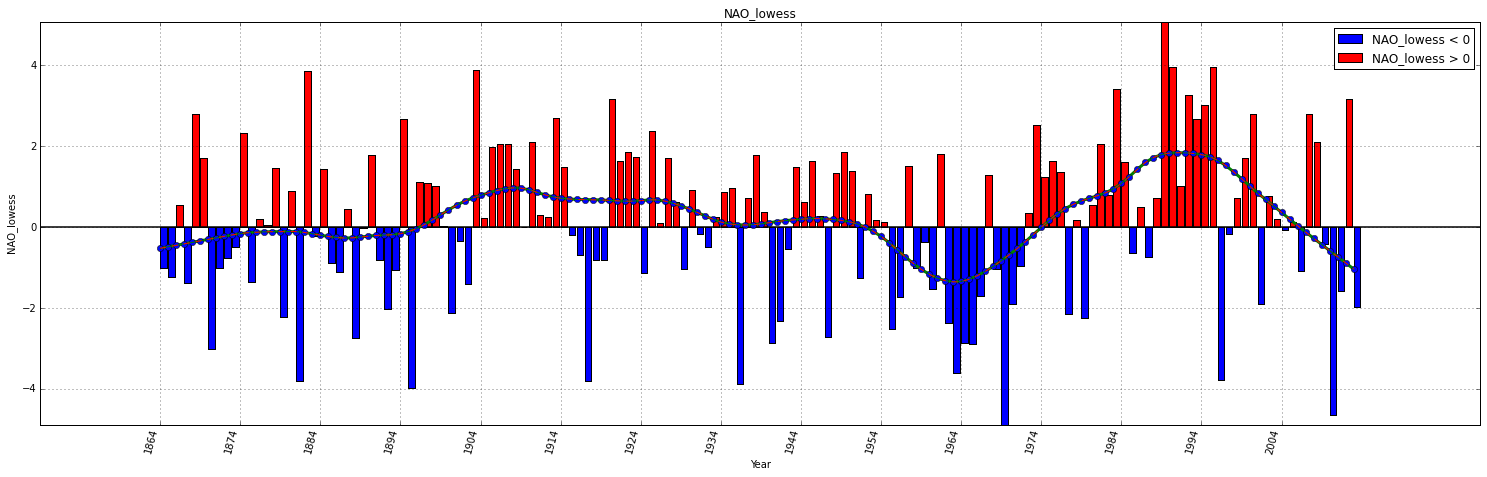
\includegraphics{NAO.png}}

{\hyperref[AMO:amo]{\emph{\DUspan{}{Atlantic Multidecadal Oscillation}}}}.


\chapter{Atlantic Multidecadal Oscillation}
\label{AMO:amo}\label{AMO:atlantic-multidecadal-oscillation}\label{AMO::doc}\begin{itemize}
\item {} 
Enable inline printing

\end{itemize}


\bigskip\hrule{}\bigskip


\begin{Verbatim}[commandchars=\\\{\}]
\PYGZpc{}matplotlib inline
\end{Verbatim}
\begin{itemize}
\item {} 
Import the cfData, cfPlot classes from the ecoop library

\end{itemize}


\bigskip\hrule{}\bigskip


\begin{Verbatim}[commandchars=\\\{\}]
\PYG{k+kn}{from} \PYG{n+nn}{ecoop.cf} \PYG{k+kn}{import} \PYG{n}{cfData}\PYG{p}{,} \PYG{n}{cfPlot}
\end{Verbatim}

\begin{Verbatim}[commandchars=\\\{\}]
\PYG{n}{cfd} \PYG{o}{=} \PYG{n}{cfData}\PYG{p}{(}\PYG{p}{)}
\PYG{n}{cfp} \PYG{o}{=} \PYG{n}{cfPlot}\PYG{p}{(}\PYG{p}{)}
\end{Verbatim}
\begin{itemize}
\item {} 
Retrieve the Atlantic Multidecadal Oscillation dataset

\end{itemize}


\bigskip\hrule{}\bigskip


\begin{Verbatim}[commandchars=\\\{\}]
\PYG{n}{amodata} \PYG{o}{=} \PYG{n}{cfd}\PYG{o}{.}\PYG{n}{amo\PYGZus{}get}\PYG{p}{(}\PYG{n}{prov}\PYG{o}{=}\PYG{n+nb+bp}{True}\PYG{p}{)}
\end{Verbatim}

\begin{Verbatim}[commandchars=\\\{\}]
dataset used: http://www.cdc.noaa.gov/Correlation/amon.us.long.data
\end{Verbatim}

\begin{Verbatim}[commandchars=\\\{\}]
\PYG{l+s}{\PYGZsq{}}\PYG{l+s}{cell\PYGZhy{}output metadata saved}\PYG{l+s}{\PYGZsq{}}
\end{Verbatim}
\begin{itemize}
\item {} 
Plot the Atlantic Multidecadal Oscillation dataset

\end{itemize}


\bigskip\hrule{}\bigskip


\begin{Verbatim}[commandchars=\\\{\}]
\PYG{c}{\PYGZsh{} NAO}
\PYG{n}{cfp}\PYG{o}{.}\PYG{n}{plot\PYGZus{}index}\PYG{p}{(}\PYG{n}{name}\PYG{o}{=}\PYG{l+s}{\PYGZsq{}}\PYG{l+s}{AMO\PYGZus{}lowess}\PYG{l+s}{\PYGZsq{}}\PYG{p}{,} \PYG{n}{xticks}\PYG{o}{=}\PYG{l+m+mi}{10}\PYG{p}{,} \PYG{n}{xticks\PYGZus{}fontsize}\PYG{o}{=}\PYG{l+m+mi}{10}\PYG{p}{,}
               \PYG{n}{data}\PYG{o}{=}\PYG{n}{amodata}\PYG{p}{,} \PYG{n}{nb}\PYG{o}{=}\PYG{l+s}{\PYGZsq{}}\PYG{l+s}{y}\PYG{l+s}{\PYGZsq{}}\PYG{p}{,} \PYG{n}{scategory}\PYG{o}{=}\PYG{l+s}{\PYGZsq{}}\PYG{l+s}{lowess}\PYG{l+s}{\PYGZsq{}}\PYG{p}{,} \PYG{n}{frac}\PYG{o}{=}\PYG{l+m+mf}{1.}\PYG{o}{/}\PYG{l+m+mi}{6}\PYG{p}{,} \PYG{n}{it}\PYG{o}{=}\PYG{l+m+mi}{6}\PYG{p}{,}
               \PYG{n}{dateformat}\PYG{o}{=}\PYG{n+nb+bp}{True}\PYG{p}{)}
\end{Verbatim}

\begin{Verbatim}[commandchars=\\\{\}]
Session output file \PYGZsq{}subplots.html\PYGZsq{} already exists, will be overwritten.
\end{Verbatim}

\scalebox{0.500000}{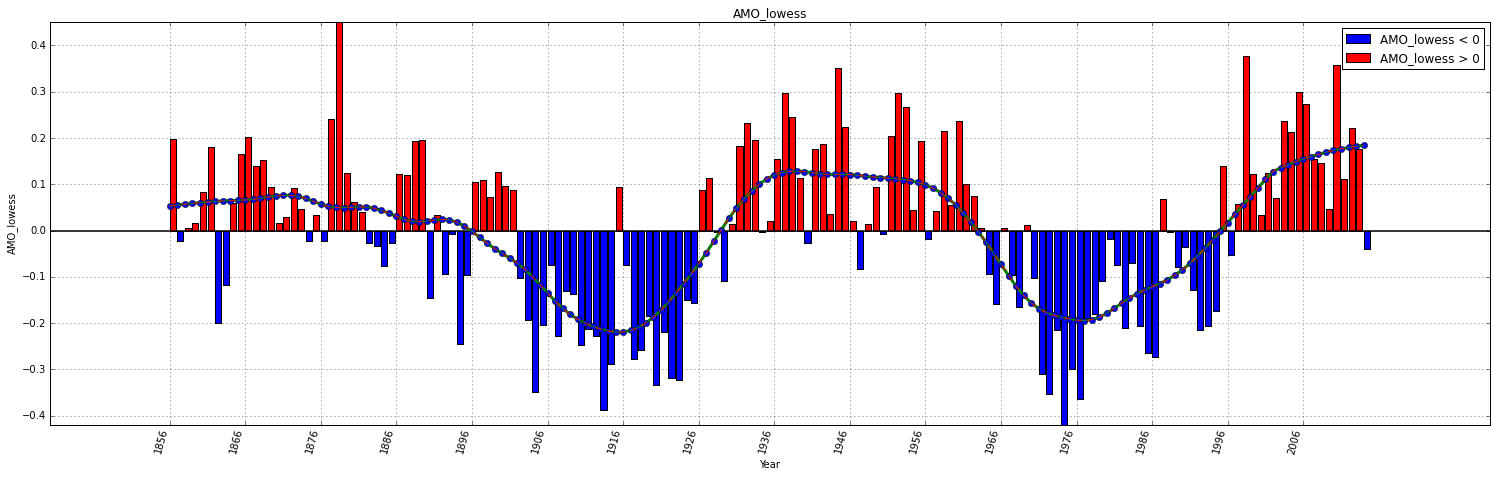
\includegraphics{AMO.png}}

{\hyperref[make_pdf:make-pdf]{\emph{\DUspan{}{Build a PDF}}}}.


\chapter{Build a PDF}
\label{make_pdf:make-pdf}\label{make_pdf::doc}\label{make_pdf:build-a-pdf}\begin{itemize}
\item {} 
Import libraries

\end{itemize}


\bigskip\hrule{}\bigskip


\begin{Verbatim}[commandchars=\\\{\}]
\PYG{k+kn}{import} \PYG{n+nn}{os}
\PYG{k+kn}{from} \PYG{n+nn}{ecoop.ecooputil} \PYG{k+kn}{import} \PYG{n}{shareUtil}
\PYG{k+kn}{from} \PYG{n+nn}{ecoop.printer} \PYG{k+kn}{import} \PYG{n}{openDocument}\PYG{p}{,} \PYG{n}{closeDocument}\PYG{p}{,} \PYG{n}{addSection}\PYG{p}{,} \PYG{n}{addSubSection}\PYG{p}{,} \PYG{n}{addFigure}
\PYG{k+kn}{from} \PYG{n+nn}{ecoop.epimagic} \PYG{k+kn}{import} \PYG{o}{*}
\end{Verbatim}

\begin{Verbatim}[commandchars=\\\{\}]
\PYGZpc{}matplotlib inline
\end{Verbatim}

\begin{Verbatim}[commandchars=\\\{\}]
\PYG{n}{util} \PYG{o}{=} \PYG{n}{shareUtil}\PYG{p}{(}\PYG{p}{)}
\end{Verbatim}
\begin{itemize}
\item {} 
Start to write the latex Document

\end{itemize}


\bigskip\hrule{}\bigskip


\begin{Verbatim}[commandchars=\\\{\}]
\PYG{n}{ID} \PYG{o}{=} \PYG{n}{util}\PYG{o}{.}\PYG{n}{get\PYGZus{}id}\PYG{p}{(}\PYG{l+s}{\PYGZsq{}}\PYG{l+s}{test/myfencypdf}\PYG{l+s}{\PYGZsq{}}\PYG{p}{)}
\PYG{n}{document} \PYG{o}{=} \PYG{n}{openDocument}\PYG{p}{(}\PYG{p}{)}
\end{Verbatim}

\begin{Verbatim}[commandchars=\\\{\}]
session data directory : test/myfencypdf\PYGZus{}Saturday\PYGZus{}26\PYGZus{}April\PYGZus{}2014\PYGZus{}05\PYGZus{}19\PYGZus{}46\PYGZus{}AM
\end{Verbatim}
\begin{itemize}
\item {} 
Abstract

\end{itemize}


\bigskip\hrule{}\bigskip


\begin{Verbatim}[commandchars=\\\{\}]
\PYGZpc{}\PYGZpc{}writefileref \PYGZob{}ID\PYGZcb{}/abstract.txt epinux
here is my little abstract, sorry it is really short ... but it is just a test to show you how easy is to use the IPython notebook with LaTex to build a nice PDF document.
\end{Verbatim}

\begin{Verbatim}[commandchars=\\\{\}]
Writing test/myfencypdf\PYGZus{}Saturday\PYGZus{}26\PYGZus{}April\PYGZus{}2014\PYGZus{}05\PYGZus{}19\PYGZus{}46\PYGZus{}AM/abstract.txt
\end{Verbatim}

\begin{Verbatim}[commandchars=\\\{\}]
\PYG{l+s}{\PYGZsq{}}\PYG{l+s}{added references for user epinux}\PYG{l+s}{\PYGZsq{}}
\end{Verbatim}

\begin{Verbatim}[commandchars=\\\{\}]
\PYG{n}{abstract} \PYG{o}{=} \PYG{n}{addSection}\PYG{p}{(}\PYG{n}{name}\PYG{o}{=}\PYG{l+s}{\PYGZsq{}}\PYG{l+s}{Abstract}\PYG{l+s}{\PYGZsq{}}\PYG{p}{,} \PYG{n}{data}\PYG{o}{=}\PYG{n}{os}\PYG{o}{.}\PYG{n}{path}\PYG{o}{.}\PYG{n}{join}\PYG{p}{(}\PYG{n}{ID}\PYG{p}{,}\PYG{l+s}{\PYGZsq{}}\PYG{l+s}{abstract.txt}\PYG{l+s}{\PYGZsq{}}\PYG{p}{)}\PYG{p}{)}
\end{Verbatim}
\begin{itemize}
\item {} 
First paragraph

\end{itemize}


\bigskip\hrule{}\bigskip


\begin{Verbatim}[commandchars=\\\{\}]
\PYGZpc{}\PYGZpc{}writefileref \PYGZob{}ID\PYGZcb{}/first\PYGZus{}paragraph.txt epinux
Here we are telling a story about our experience building a simple PDF document.
The text inside this cell will go in the first paragraph (chapter?) of our PDF document.
\end{Verbatim}

\begin{Verbatim}[commandchars=\\\{\}]
Writing test/myfencypdf\PYGZus{}Saturday\PYGZus{}26\PYGZus{}April\PYGZus{}2014\PYGZus{}05\PYGZus{}19\PYGZus{}46\PYGZus{}AM/first\PYGZus{}paragraph.txt
\end{Verbatim}

\begin{Verbatim}[commandchars=\\\{\}]
\PYG{l+s}{\PYGZsq{}}\PYG{l+s}{added references for user epinux}\PYG{l+s}{\PYGZsq{}}
\end{Verbatim}

\begin{Verbatim}[commandchars=\\\{\}]
\PYG{k+kn}{import} \PYG{n+nn}{numpy} \PYG{k+kn}{as} \PYG{n+nn}{np}
\PYG{k+kn}{import} \PYG{n+nn}{matplotlib.pyplot} \PYG{k+kn}{as} \PYG{n+nn}{plt}

\PYG{n}{x} \PYG{o}{=} \PYG{n}{np}\PYG{o}{.}\PYG{n}{array}\PYG{p}{(}\PYG{p}{[}\PYG{l+m+mi}{1}\PYG{p}{,}\PYG{l+m+mi}{2}\PYG{p}{,}\PYG{l+m+mi}{3}\PYG{p}{]}\PYG{p}{)}
\PYG{n}{y} \PYG{o}{=} \PYG{n}{np}\PYG{o}{.}\PYG{n}{array}\PYG{p}{(}\PYG{p}{[}\PYG{l+m+mi}{1}\PYG{p}{,}\PYG{l+m+mi}{2}\PYG{p}{,}\PYG{l+m+mi}{3}\PYG{p}{]}\PYG{p}{)}
\PYG{n}{plt}\PYG{o}{.}\PYG{n}{plot}\PYG{p}{(}\PYG{n}{x}\PYG{p}{,}\PYG{n}{y}\PYG{p}{,}\PYG{l+s}{\PYGZsq{}}\PYG{l+s}{\PYGZhy{}}\PYG{l+s}{\PYGZsq{}}\PYG{p}{)}
\PYG{n}{plt}\PYG{o}{.}\PYG{n}{xlabel}\PYG{p}{(}\PYG{l+s}{\PYGZsq{}}\PYG{l+s}{xlabels}\PYG{l+s}{\PYGZsq{}}\PYG{p}{)}
\PYG{n}{plt}\PYG{o}{.}\PYG{n}{title}\PYG{p}{(}\PYG{l+s}{\PYGZsq{}}\PYG{l+s}{myfencyplot}\PYG{l+s}{\PYGZsq{}}\PYG{p}{)}
\PYG{n}{plt}\PYG{o}{.}\PYG{n}{show}\PYG{p}{(}\PYG{p}{)}
\PYG{n}{plt}\PYG{o}{.}\PYG{n}{savefig}\PYG{p}{(}\PYG{n}{os}\PYG{o}{.}\PYG{n}{path}\PYG{o}{.}\PYG{n}{join}\PYG{p}{(}\PYG{n}{ID}\PYG{p}{,}\PYG{l+s}{\PYGZsq{}}\PYG{l+s}{myfencyplot.png}\PYG{l+s}{\PYGZsq{}}\PYG{p}{)}\PYG{p}{)}
\end{Verbatim}

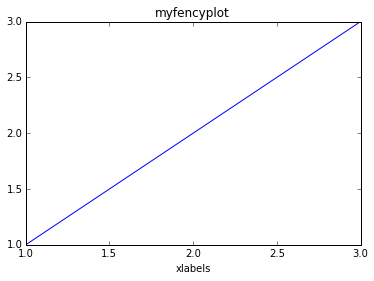
\includegraphics{myfency.png}

\begin{Verbatim}[commandchars=\\\{\}]
\PYGZlt{}matplotlib.figure.Figure at 0x7ffbeda42e10\PYGZgt{}
\end{Verbatim}

\begin{Verbatim}[commandchars=\\\{\}]
\PYG{n}{fig1} \PYG{o}{=} \PYG{n}{addFigure}\PYG{p}{(}\PYG{n}{img}\PYG{o}{=}\PYG{n}{os}\PYG{o}{.}\PYG{n}{path}\PYG{o}{.}\PYG{n}{join}\PYG{p}{(}\PYG{n}{ID}\PYG{p}{,}\PYG{l+s}{\PYGZsq{}}\PYG{l+s}{myfencyplot.png}\PYG{l+s}{\PYGZsq{}}\PYG{p}{)}\PYG{p}{,} \PYG{n}{name}\PYG{o}{=}\PYG{l+s}{\PYGZsq{}}\PYG{l+s}{myfencyplot}\PYG{l+s}{\PYGZsq{}}\PYG{p}{,}\PYG{n}{metadata}\PYG{o}{=}\PYG{l+s}{\PYGZsq{}}\PYG{l+s}{\PYGZsq{}}\PYG{p}{)}
\end{Verbatim}

\begin{Verbatim}[commandchars=\\\{\}]
\PYG{n}{firstparagraph}  \PYG{o}{=} \PYG{n}{addSubSection}\PYG{p}{(}\PYG{n}{name}\PYG{o}{=}\PYG{l+s}{\PYGZsq{}}\PYG{l+s}{First paragraph}\PYG{l+s}{\PYGZsq{}}\PYG{p}{,} \PYG{n}{data}\PYG{o}{=}\PYG{n}{os}\PYG{o}{.}\PYG{n}{path}\PYG{o}{.}\PYG{n}{join}\PYG{p}{(}\PYG{n}{ID}\PYG{p}{,}\PYG{l+s}{\PYGZsq{}}\PYG{l+s}{first\PYGZus{}paragraph.txt}\PYG{l+s}{\PYGZsq{}}\PYG{p}{)}\PYG{p}{,} \PYG{n}{fig}\PYG{o}{=}\PYG{n}{fig1}\PYG{p}{)}
\end{Verbatim}

\begin{Verbatim}[commandchars=\\\{\}]
\PYG{n}{closedDocument} \PYG{o}{=} \PYG{n}{closeDocument}\PYG{p}{(}\PYG{p}{)}
\end{Verbatim}
\begin{itemize}
\item {} 
Write Latex Document

\end{itemize}


\bigskip\hrule{}\bigskip


\begin{Verbatim}[commandchars=\\\{\}]
\PYG{n}{texfile}\PYG{o}{=}\PYG{l+s}{\PYGZsq{}}\PYG{l+s}{\PYGZsq{}}
\PYG{n}{texfile} \PYG{o}{+}\PYG{o}{=} \PYG{n}{document}
\PYG{n}{texfile} \PYG{o}{+}\PYG{o}{=} \PYG{n}{abstract}
\PYG{n}{texfile} \PYG{o}{+}\PYG{o}{=} \PYG{n}{firstparagraph}
\PYG{n}{texfile} \PYG{o}{+}\PYG{o}{=} \PYG{n}{closedDocument}
\end{Verbatim}

\begin{Verbatim}[commandchars=\\\{\}]
\PYG{n}{pdf} \PYG{o}{=} \PYG{n}{os}\PYG{o}{.}\PYG{n}{path}\PYG{o}{.}\PYG{n}{join}\PYG{p}{(}\PYG{n}{ID}\PYG{p}{,}\PYG{l+s}{\PYGZsq{}}\PYG{l+s}{test.tex}\PYG{l+s}{\PYGZsq{}}\PYG{p}{)}
\PYG{n}{f} \PYG{o}{=} \PYG{n+nb}{open}\PYG{p}{(}\PYG{n}{pdf}\PYG{p}{,}\PYG{l+s}{\PYGZsq{}}\PYG{l+s}{w}\PYG{l+s}{\PYGZsq{}}\PYG{p}{)}
\PYG{n}{f}\PYG{o}{.}\PYG{n}{write}\PYG{p}{(}\PYG{n}{texfile}\PYG{p}{)}
\PYG{n}{f}\PYG{o}{.}\PYG{n}{close}\PYG{p}{(}\PYG{p}{)}
\end{Verbatim}
\begin{itemize}
\item {} 
Build PDF

\end{itemize}


\bigskip\hrule{}\bigskip


\begin{Verbatim}[commandchars=\\\{\}]
!pdflatex \PYGZhy{}output\PYGZhy{}directory=\PYGZob{}ID\PYGZcb{} \PYGZob{}pdf\PYGZcb{}
\end{Verbatim}
\begin{alltt}
This is pdfTeX, Version 3.1415926-2.4-1.40.13 (TeX Live 2012/Debian)
 restricted write18 enabled.
entering extended mode
(./test/myfencypdf\_Saturday\_26\_April\_2014\_05\_19\_46\_AM/test.tex
LaTeX2e \textless{}2011/06/27\textgreater{}
Babel \textless{}v3.8m\textgreater{} and hyphenation patterns for english, dumylang, nohyphenation, et
hiopic, farsi, arabic, pinyin, croatian, bulgarian, ukrainian, russian, slovak,
 czech, danish, dutch, usenglishmax, ukenglish, finnish, french, basque, ngerma
n, german, swissgerman, ngerman-x-2012-05-30, german-x-2012-05-30, monogreek, g
reek, ibycus, ancientgreek, hungarian, bengali, tamil, hindi, telugu, gujarati,
 sanskrit, malayalam, kannada, assamese, marathi, oriya, panjabi, italian, lati
n, latvian, lithuanian, mongolian, mongolianlmc, nynorsk, bokmal, indonesian, e
speranto, coptic, welsh, irish, interlingua, serbian, serbianc, slovenian, friu
lan, romansh, estonian, romanian, armenian, uppersorbian, turkish, afrikaans, i
celandic, kurmanji, polish, portuguese, galician, catalan, spanish, swedish, th
ai, loaded.
(/usr/share/texlive/texmf-dist/tex/latex/base/article.cls
Document Class: article 2007/10/19 v1.4h Standard LaTeX document class
(/usr/share/texlive/texmf-dist/tex/latex/base/size10.clo))
(/usr/share/texlive/texmf-dist/tex/latex/tools/multicol.sty)
(/var/lib/texmf/tex/generic/babel/babel.sty
(/usr/share/texlive/texmf-dist/tex/generic/babel/english.ldf
(/usr/share/texlive/texmf-dist/tex/generic/babel/babel.def)))
(/usr/share/texlive/texmf-dist/tex/latex/blindtext/blindtext.sty
(/usr/share/texlive/texmf-dist/tex/latex/tools/xspace.sty))
(/usr/share/texlive/texmf-dist/tex/latex/graphics/graphicx.sty
(/usr/share/texlive/texmf-dist/tex/latex/graphics/keyval.sty)
(/usr/share/texlive/texmf-dist/tex/latex/graphics/graphics.sty
(/usr/share/texlive/texmf-dist/tex/latex/graphics/trig.sty)
(/usr/share/texlive/texmf-dist/tex/latex/latexconfig/graphics.cfg)
(/usr/share/texlive/texmf-dist/tex/latex/pdftex-def/pdftex.def
(/usr/share/texlive/texmf-dist/tex/generic/oberdiek/infwarerr.sty)
(/usr/share/texlive/texmf-dist/tex/generic/oberdiek/ltxcmds.sty))))
(/usr/share/texlive/texmf-dist/tex/latex/wrapfig/wrapfig.sty)
(/usr/share/texlive/texmf-dist/tex/latex/hyperref/hyperref.sty
(/usr/share/texlive/texmf-dist/tex/generic/oberdiek/hobsub-hyperref.sty
(/usr/share/texlive/texmf-dist/tex/generic/oberdiek/hobsub-generic.sty))
(/usr/share/texlive/texmf-dist/tex/generic/ifxetex/ifxetex.sty)
(/usr/share/texlive/texmf-dist/tex/latex/oberdiek/kvoptions.sty)
(/usr/share/texlive/texmf-dist/tex/latex/hyperref/pd1enc.def)
(/usr/share/texlive/texmf-dist/tex/latex/latexconfig/hyperref.cfg)
(/usr/share/texlive/texmf-dist/tex/latex/url/url.sty))

Package hyperref Message: Driver (autodetected): hpdftex.

(/usr/share/texlive/texmf-dist/tex/latex/hyperref/hpdftex.def
(/usr/share/texlive/texmf-dist/tex/latex/oberdiek/rerunfilecheck.sty))
(/usr/share/texlive/texmf-dist/tex/latex/fancyvrb/fancyvrb.sty
Style option: {\color{red}\bfseries{}{}`}fancyvrb' v2.7a, with DG/SPQR fixes, and firstline=lastline fix
\textless{}2008/02/07\textgreater{} (tvz)) (/usr/share/texlive/texmf-dist/tex/latex/base/inputenc.sty
(/usr/share/texlive/texmf-dist/tex/latex/base/utf8.def
(/usr/share/texlive/texmf-dist/tex/latex/base/t1enc.dfu)
(/usr/share/texlive/texmf-dist/tex/latex/base/ot1enc.dfu)
(/usr/share/texlive/texmf-dist/tex/latex/base/omsenc.dfu))) (./test.aux)
(/usr/share/texlive/texmf-dist/tex/context/base/supp-pdf.mkii
{[}Loading MPS to PDF converter (version 2006.09.02).{]}
) (/usr/share/texlive/texmf-dist/tex/latex/oberdiek/epstopdf-base.sty
(/usr/share/texlive/texmf-dist/tex/latex/oberdiek/grfext.sty)
(/usr/share/texlive/texmf-dist/tex/latex/latexconfig/epstopdf-sys.cfg))
(/usr/share/texlive/texmf-dist/tex/latex/hyperref/nameref.sty
(/usr/share/texlive/texmf-dist/tex/generic/oberdiek/gettitlestring.sty))
(./test.out) (./test.out)
(./test/myfencypdf\_Saturday\_26\_April\_2014\_05\_19\_46\_AM/abstract.txt)
(./test/myfencypdf\_Saturday\_26\_April\_2014\_05\_19\_46\_AM/first\_paragraph.txt)
\textless{}test/myfencypdf\_Saturday\_26\_April\_2014\_05\_19\_46\_AM/myfencyplot.png, id=4, 433.
62pt x 289.08pt\textgreater{}
\textless{}use test/myfencypdf\_Saturday\_26\_April\_2014\_05\_19\_46\_AM/myfencyplot.png\textgreater{}
Overfull hbox (3.21652pt too wide) in paragraph at lines 19--20
{[}{]}{[}{]}

Package hyperref Warning: Empty destination name,
(hyperref)                using {\color{red}\bfseries{}{}`}UNDEFINED' on input line 20.

{[}1\{/var/lib/texmf/fonts/map/pdftex/updmap/pdftex.map\} \textless{}./test/myfencypdf\_Saturd
ay\_26\_April\_2014\_05\_19\_46\_AM/myfencyplot.png\textgreater{}{]}
(test/myfencypdf\_Saturday\_26\_April\_2014\_05\_19\_46\_AM/test.aux) )
(see the transcript file for additional information)pdfTeX warning (dest): name
\{UNDEFINED\} has been referenced but does not exist, replaced by a fixed one

\textless{}/usr/share/texlive/texmf-dist/fonts/type1/public/amsfonts/cm/cmbx12.pfb\textgreater{}\textless{}/usr/
share/texlive/texmf-dist/fonts/type1/public/amsfonts/cm/cmr10.pfb\textgreater{}
Output written on test/myfencypdf\_Saturday\_26\_April\_2014\_05\_19\_46\_AM/test.pdf (
1 page, 29584 bytes).
Transcript written on test/myfencypdf\_Saturday\_26\_April\_2014\_05\_19\_46\_AM/test.l
og.
\end{alltt}
\phantomsection\label{index:module-ecoop}\index{ecoop (module)}

\chapter{Indices and tables}
\label{index:indices-and-tables}\begin{itemize}
\item {} 
\DUspan{xref,std,std-ref}{genindex}

\item {} 
\DUspan{xref,std,std-ref}{modindex}

\item {} 
\DUspan{xref,std,std-ref}{search}

\end{itemize}


\renewcommand{\indexname}{Python Module Index}
\begin{theindex}
\def\bigletter#1{{\Large\sffamily#1}\nopagebreak\vspace{1mm}}
\bigletter{e}
\item {\texttt{ecoop}}, \pageref{index:module-ecoop}
\end{theindex}

\renewcommand{\indexname}{Index}
\printindex
\end{document}
